\documentclass[12pt]{article}
\usepackage{amsmath}
\usepackage{amssymb}
\usepackage{graphicx}
\usepackage[round,sort]{natbib}
\DeclareMathOperator*{\argmin}{arg\,min}
\graphicspath{ {../img/}{../img/au/} {../img/us/}{../img/in/}{../img/stringency_index/}}
\begin{document}
		\section{Introduction}
		\label{SEC1}
			\subsection{Related Works}
		Other modeling approaches. SIR-F, DCM, Agent, Hybrid - not post fact A/B testing tools.
		
		\subsection{Tools}
		As stated above, our objective is to study the effects of government response at an aggregate level in terms of life saved, and limiting the number of cases that requires hospitalization. Such interventions can effectively be studied at a comparative level. In other words, if we have data for the evolution of aggregate outcomes, e.g. number of confirmed cases and deaths, when policy is applied in a group under study versus when the same policy is not applied in a control group. However, government policies were applied at different level across a geographic region.  We do not have a mechanism to conduct a randomized trial. Hence, we consider constructing synthetic control method\cite{ap08746, JMLR18, AMSS19}. In a synthetic control set up, where observational data is available for different groups, we can construct a synthetic or virtual control group by combining measurements from alternatives (or donors). In following we provide a brief overview of Multi-dimensional Robust Synthetic Control following\cite{AMSS19}.\par
		
		Suppose that observations from $N$ different geographically distinct groups or units are indexed by $i \in [N]$ in $T$ time periods (days) indexed by $j \in [T]$. Let $k \in [K]$ be the metrics of interest (e.g. number of confirmed cases, number of deaths, number of tests conducted, etc.). By $M_{ijk}$ we denote the ground-truth measurement of interest, and by $X_{ijk}$, an observation of this measurement with some noise. Let $1 \leq T_0 \leq T$ be the time instance in which our group of interest experiences an intervention, namely a government response to control the spread (e.g. stay home order, school or business closure, or mass vaccination). Without loss of generality we consider unit $i = 1$ (say, New York) and metric $k = 1$ (say, number of deaths) as our unit and metric of interest respectively.\par
		
		Our objective now is to estimate the trajectory of metric of interest $k = 1$  for unit $i = 1$ if no government response to control the spread had occurred. In order to do that we will use the trajectory associated with the donor units ($2 \leq i \leq N$ ), and metrics $k \in [K ]$. In following we make two assumptions: (1) for all $2 \leq i \leq N$, $k \in [K]$ and $j \in [T]$, we have  $X_{ijk} = M_{ijk} + \epsilon_{ijk}$ where, $\epsilon_{ijk}$ is the observational noise, and (2) Same model is obeyed by $i=1$ in pre--intervention period, i.e. for all $j \in [T_0]$ and $k \in [K]$ we have $X_{1jk} = M_{1jk} + \epsilon_{1jk}$. As described by authors in \cite{AMSS19}, in following we also assume that for unit $i=1$, we only observe the measurement $X_{1jk}$ for pre-intervention period, i.e. for all $j \in [T_0]$ and $k \in [K]$. Our objective is to compute a counterfactual sequence of observation $M_{1jk}$ for the time period $j \in [T]$, and $k \in [K]$, and in specific for $T_0 \leq j \leq T$, and $k = 1$, using synthetic version of unit $i=1$.\par
		
		Define $\mathcal{M} = [M_{ijk}] \in \mathbb{R}^{N \times T \times K}$. $\mathcal{M}$ is assumed to have a few well behaved properties as required by the algorithm, namely, it must be approximately low-rank and boundedness of $\left|M_{ijk}\right|$ (for details see \cite{AMSS19}). To check whether our model assumption holds in practice, we consider $N=185, T=150, K=2$, with $185$ countries as units. We consider number of confirmed cases and number of deceased as two metrics over $150$ days between January 22, 2020 and June 20, 2020. For assumption to hold, data matrix corresponding to number of confirmed cases and number of deceased and their combination should be approximated by a low-rank matrix. 
		
		\begin{figure}[ht]
			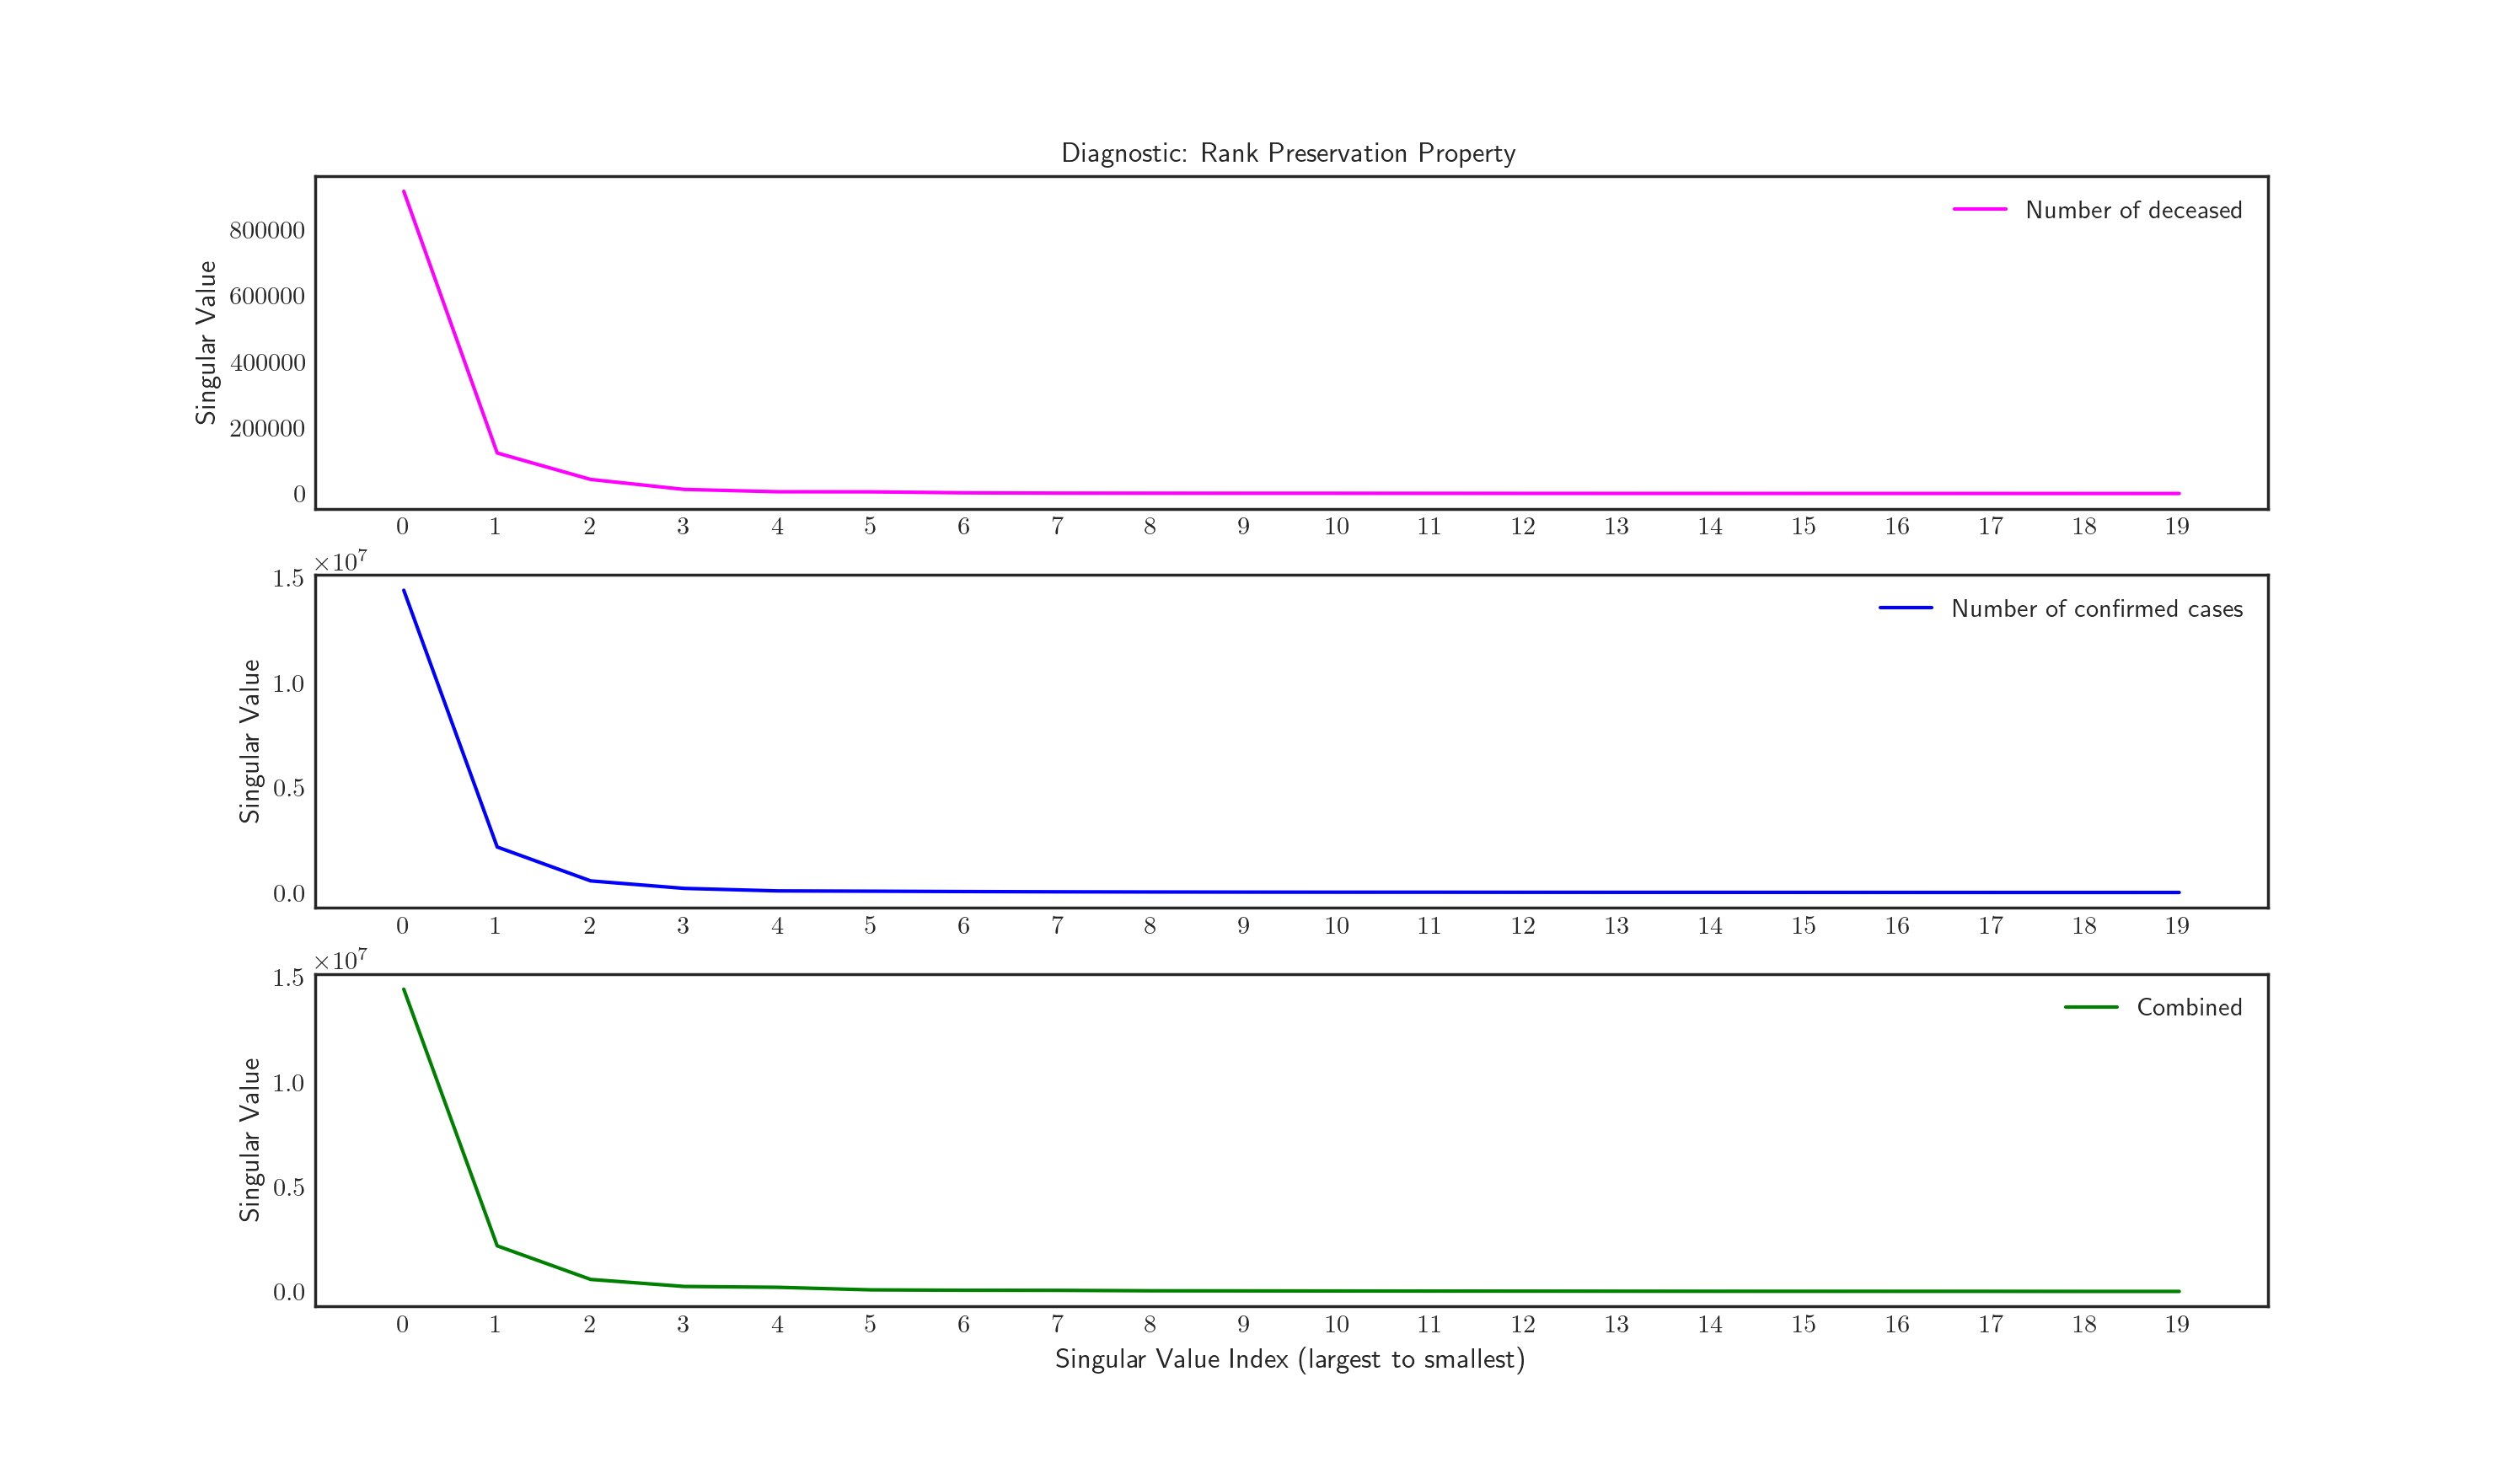
\includegraphics[width=\textwidth]{rd}
			\caption{The Singular Value spectrum for all countries (of dimensions 185 × 150, showing top 20 singular values, in descending order.} 
			\label{fig1} 
		\end{figure}
	
		As shown in Figure \ref{fig1}, the spectrum of the top 20 singular values (sorted in descending order) for each matrix. The plots clearly support the implications that most of the spectrum is concentrated within the top 5 principal components. Same conclusion holds true when units are states of United States, and when we consider only countries in European Union.\par
		
		Let $\mathcal{Z} \in \mathbb{R}^{(N-1) \times T \times K}$ corresponding to donor units, and $X_1 \in \mathbb{R}^{1 \times T_0 \times K}$ correspond to unit under intervention. We obtain $\hat{\mathcal{M}}$ from $\mathcal{Z}$ after applying a hard singular value thresholding. Subsequently, weights are learned using linear regression by computing
		
		\begin{equation*}
			\hat{\beta} = \argmin_{v \in \mathbb{R}^{(N-1)} } \left\| X_1 - v^T \hat{\mathcal{M}}_{T_0}\right\|^2_2
		\end{equation*}
        
        For every $k \in [K]$, the corresponding estimated counterfactual means for the treatment unit is then defined as
        
        \begin{equation*}
        \hat{\mathcal{M}}_1^{(k)} = \hat{\beta}^T \hat{\mathcal{M}}^{(k)}
        \end{equation*}
        
		\section{Methods}
		\label{SEC2}
		\subsection{Overview}
		As described in Section \ref{SEC1}, we use Multi-dimensional Robust Synthetic Control to construct a synthetic control for the treatment unit using data from multiple control units or donor group using pre-intervention period data.  The synthetic control is then used for estimating the counterfactual in the post-intervention period. In our setup intervention date is typically the date when a stay-home order or lock-down was declared for the treatment unit.  However, government policy may have been applied over time with different level of stringency measures. 
		
		To understand this we use stringency and policy indices data from OxCGRT \cite{HWP2020}, which records the strictness of policies that restrict people’s behavior and includes 8 different measures - e.g. school  and workplace closure, cancellation of public events, restrictions on gathering size etc. As 
		
		\subsection{Data Source}
		
		\subsection{Setup}
		
		
		\section{Results}
		\label{SEC3}
		
		\section{Discussion}
		\label{SEC4}
		
		
		\section{Concluding Remarks}
		\label{SEC5}
		%% References
		
		\bibliographystyle{abbrvnat}
		\bibliography{lockdown.bib}	
	\end{document}